%!TEX root = main.tex
\section{Discussion}



% % \begin{wrapfigure}{R}{0.5\textwidth}
\begin{figure}[!t]
% \centering
\floatbox[{\capbeside\thisfloatsetup{capbesideposition={left},capbesidewidth=6cm}}]{figure}[\FBwidth]
{
\begin{tabular}{c@{\extracolsep{\fill}}ccc}
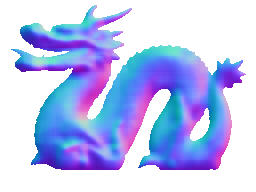
\includegraphics[width=0.32\linewidth]{figures/results/uniform_output_crop.png} &
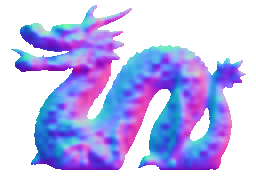
\includegraphics[width=0.32\linewidth]{figures/results/checker_normal_small_20160617_21_output_crop.png} &
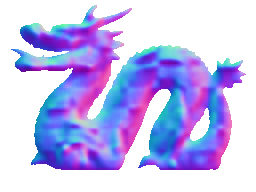
\includegraphics[width=0.32\linewidth]{figures/results/checker_normal_large_20160617_21_output_crop.png} \\
%
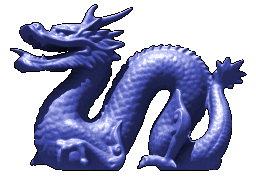
\includegraphics[width=0.32\linewidth]{figures/results/uniform_input_gray_color_crop.png} &
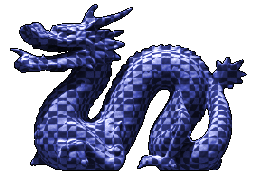
\includegraphics[width=0.32\linewidth]{figures/results/checker_small_input_gray_color_crop.png} &
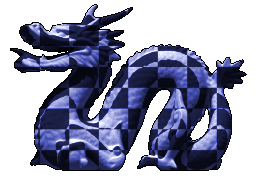
\includegraphics[width=0.32\linewidth]{figures/results/checker_large_input_gray_color_crop.png} 
\end{tabular}
}
{\caption{Limitation of our approach. Our network is trained on spatially uniform BRDFs, so testing it on spatially-varying albedo maps increases the estimation error. (left) Spatially-uniform albedos results in low error, while checkerboard albedo maps with (center) small and (right) large patterns increase the error.}\label{fig:limitations}}
\end{figure}


In this chapter, we present what we believe to be the first learned single-day photometric stereo method. Two key ideas were used to train our approach: first, local spatiality is important in the single-day case and can be leveraged using convolutional layers; second, large synthetic data with different surface reflectance can generalize well to real lighting and allows the training of deep learning methods. This results in a method robust to shadows, specular highlights and different albedos. We show that our method significantly outperforms previous work on a challenging evaluation dataset of virtual objects lit by real sunny lighting conditions.

Despite offering state-of-the-art performance, our method suffers from some limitations, which opens the way for interesting future work. The first limitation is that the camera is assumed to be pointing north. Although the network shows some resilience to errors in camera calibration (see fig.~\ref{fig:calibration_error_performance}), large deviations from the assumed direction are not well-handled. One possible way to circumvent this limitation would be to train direction-specific models and select the right one by detecting the camera orientation. Furthermore, while our approach is robust to non-Lambertian reflections, it assumes the scene to have a spatially-uniform BRDF. Fig.~\ref{fig:limitations} shows the behavior of our approach when the object is texture mapped with two spatially-varying albedo maps: a checkerboard pattern with small and large squares. Unsurprisingly, the resulting normal maps appear distorted since the constant albedo assumption is broken. One interesting direction for future work here would be to train a network on the \emph{ratio} between pairs of images (e.g. as in~\cite{yu-iccp-13}), which effectively cancels out the albedo. Lastly, we chose to focus on sunny days, since this is the most challenging case for outdoor photometric stereo~\cite{holdgeoffroy-iccp-15,holdgeoffroy-3dv-15}. Training the network on partially-cloudy days (for instance, by increasing the turbidity of the Ho\v{s}ek-Wilkie model) would be one potential way forward. 



% \section{Acknowledgements}




% To further understand the impact of non-uniform albedo on our approach, we applied a spatially-varying albedo to the the real lighting dataset used in evaluation. Two diffuse checkerboard patterns of different sizes were used as material. The checkerboard pattern sizes were chosen to be smaller and larger than the receptive field of our CNN. The dark squares from the checkerboard pattern have a gray albedo of 0.2 while the bright squares use the albedo sampling method described in sec.~\ref{sec:evaluation_dataset}. The results on this dataset are shown in fig.~\ref{fig:checker_experiments}. A loss of performance on the dataset median of roughly 3 and 5 degrees can be observe for the small and large checkerboard pattern, respectively. Qualitatively, our approach seems to assign a downward normal to the dark regions of the checkerboard pattern, as to explain the low pixel intensity by assuming it is facing the ground.




% \begin{figure}[!t]
% \centering
% \begin{tabular}{c@{\extracolsep{\fill}}ccc}
% 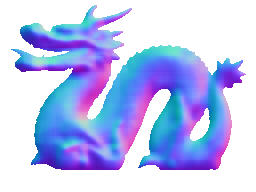
\includegraphics[width=0.2\linewidth]{figures/results/uniform_output_crop.png} &
% 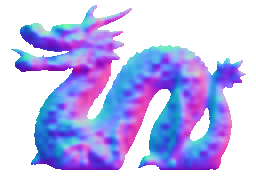
\includegraphics[width=0.2\linewidth]{figures/results/checker_normal_small_20160617_21_output_crop.png} &
% 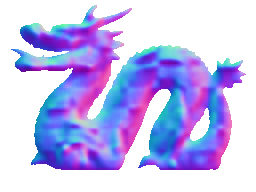
\includegraphics[width=0.2\linewidth]{figures/results/checker_normal_large_20160617_21_output_crop.png} \\
% %
% 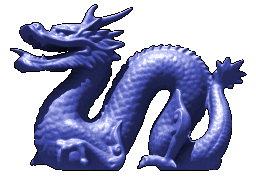
\includegraphics[width=0.2\linewidth]{figures/results/uniform_input_gray_color_crop.png} &
% 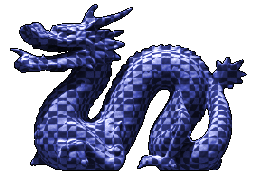
\includegraphics[width=0.2\linewidth]{figures/results/checker_small_input_gray_color_crop.png} &
% 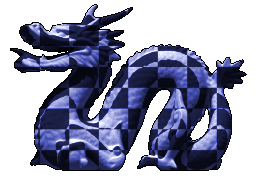
\includegraphics[width=0.2\linewidth]{figures/results/checker_large_input_gray_color_crop.png} \\
% (a) & (b) & (c)
% \end{tabular} \\
% \caption{Limitation of our approach. Our network is trained on spatially uniform BRDFs, so testing it on spatially-varying albedo maps increases the estimation error. (a) Quantiative comparison on our evaluation test set. (b) Spatially-uniform albedos results in low error, while checkerboard albedo maps with (c) small and (d) large patterns increase the error.}
% \label{fig:limitations}
% \end{figure}


% \begin{figure}[!t]
% \centering
% \begin{tabular}{c@{\extracolsep{\fill}}cccc}
% \multirow{2}{*}[4.5em]{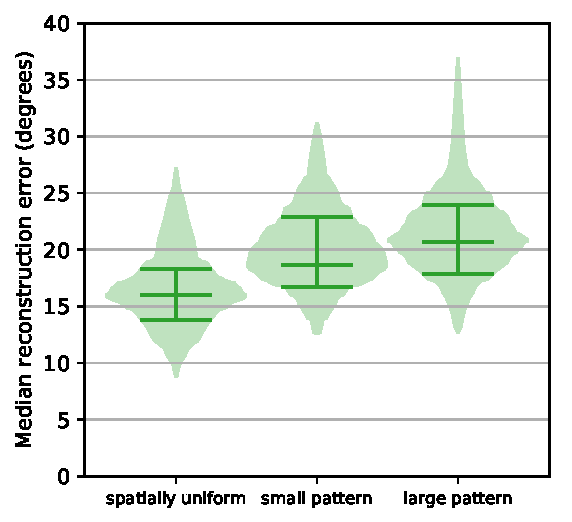
\includegraphics[width=0.35\linewidth]{figures/results/checker_experiments.pdf}} &
% 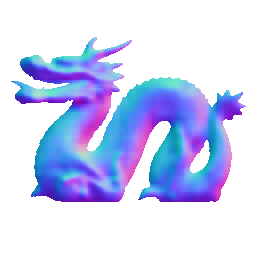
\includegraphics[width=0.2\linewidth]{figures/results/uniform_output.png} &
% 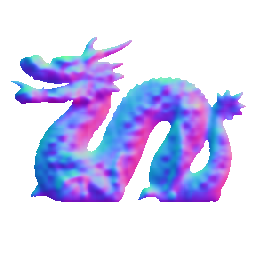
\includegraphics[width=0.2\linewidth]{figures/results/checker_normal_small_20160617_21_output.png} &
% 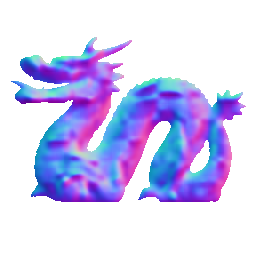
\includegraphics[width=0.2\linewidth]{figures/results/checker_normal_large_20160617_21_output.png} \\
% %
% & 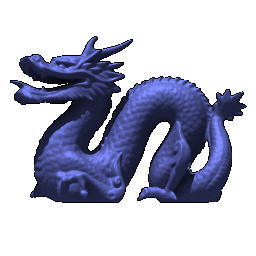
\includegraphics[width=0.2\linewidth]{figures/results/uniform_input_gray_color.png} &
% 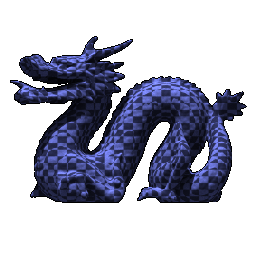
\includegraphics[width=0.2\linewidth]{figures/results/checker_small_input_gray_color.png} &
% 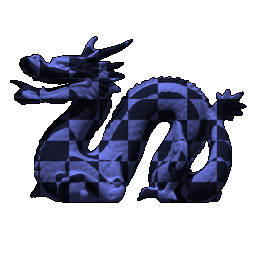
\includegraphics[width=0.2\linewidth]{figures/results/checker_large_input_gray_color.png} \\
% (a) & (b) & (c) & (d)
% \end{tabular} \\
% \caption{Limitation of our approach. Our network is trained on spatially uniform BRDFs, so testing it on spatially-varying albedo maps increases the estimation error. (a) Quantiative comparison on our evaluation test set. (b) Spatially-uniform albedos results in low error, while checkerboard albedo maps with (c) small and (d) large patterns increase the error.}
% \label{fig:limitations}
% \end{figure}

% \begin{figure}[!t]
% \centering
% \begin{tabular}{c@{\extracolsep{\fill}}cccc}
% \multirow{2}{*}[4.5em]{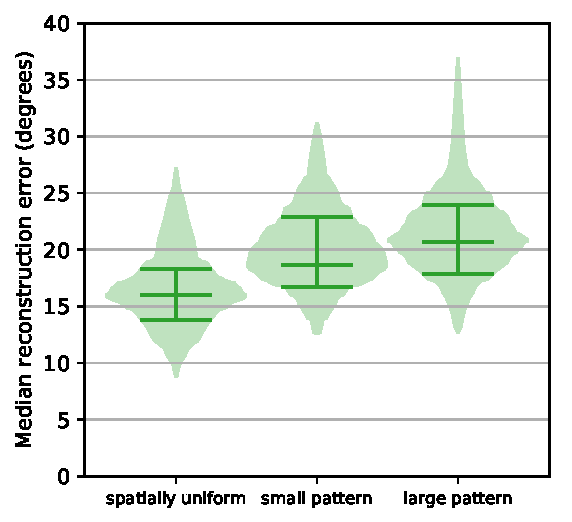
\includegraphics[width=0.35\linewidth]{figures/results/checker_experiments.pdf}} &
% 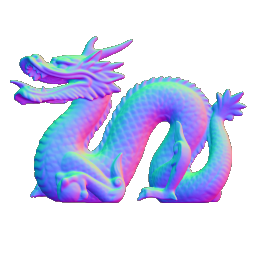
\includegraphics[width=0.18\linewidth]{figures/results/checker_20160617_21_gt.png} &
% 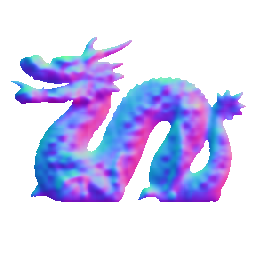
\includegraphics[width=0.18\linewidth]{figures/results/checker_normal_small_20160617_21_output.png} &
% 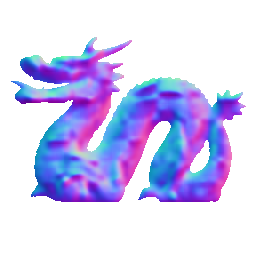
\includegraphics[width=0.18\linewidth]{figures/results/checker_normal_large_20160617_21_output.png} &
% \rotatebox[origin=l]{90}{\hspace{1.1em}normals} \\
% & 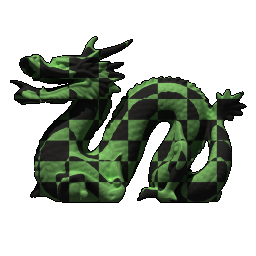
\includegraphics[width=0.18\linewidth]{figures/results/checker_large_input.png} &
% 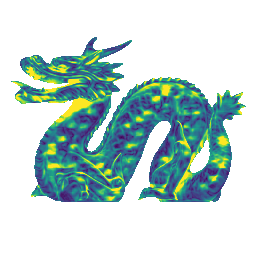
\includegraphics[width=0.18\linewidth]{figures/results/checker_normal_small_20160617_21_error.png} &
% 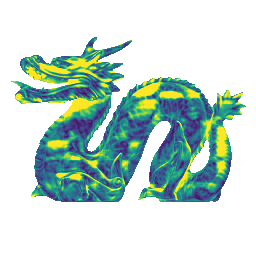
\includegraphics[width=0.18\linewidth]{figures/results/checker_normal_large_20160617_21_error.png} &
% 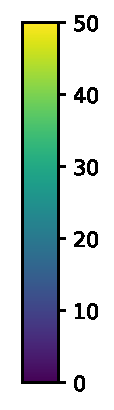
\includegraphics[height=60pt]{figures/results/checker_colorbar_error_vertical.pdf}
% \rotatebox[origin=l]{90}{\hspace{2em}error} \\
% (a) & (b) & (c) & (d)
% \end{tabular} \\
% \caption{Evaluation on objects with non-uniform albedos. (a) Median reconstruction error in degrees of our method spatially uniform albedo maps (left), small and large checkerboard patterns (center and right) over our evaluation dataset. The ground truth normal map and example input image with a large checkerboard pattern are shown in (b). Qualitative normal recovery results and errors in degrees are shown for the small pattern (c) and large pattern (d).}
% \label{fig:checker_experiments}
% \end{figure}

